\documentclass[11pt,twoside,a4paper]{article}
\title{Maths Notes for 2022 Exam}
% Open Sans font for the whole document
\usepackage[default]{opensans}
\usepackage[T1]{fontenc}
\usepackage[a4paper, margin=1.91cm, top=2.91cm, bottom=2.91cm]{geometry}
\usepackage[utf8]{inputenc}
\usepackage{pdfpages}
\usepackage{endnotes}
\usepackage{lipsum}
% Maths symbols and packages
\usepackage{amsmath}
\usepackage{amssymb}
\usepackage{fancyhdr}
\usepackage{multicol}
\pagestyle{fancy}
\fancyhf{}
\setlength{\headheight}{15.2pt}
\fancyhead[LE,RO]{ NEA Analysis }
\fancyfoot[LE,RO]{ \thepage }
\fancyfoot[RE,LO]{ \textit{Max Bowman 2021} }
\usepackage{mdframed}
\newmdtheoremenv[linewidth = 1pt]{theorem}{Theorem}
\usepackage{refcount}
\newcommand{\pagedifference}[2]{%
  \number\numexpr\getpagerefnumber{#2}-\getpagerefnumber{#1}\relax}
%stuff for graphs etc
\usepackage{tikz}
\usepackage{tkz-euclide}
\usepackage{pgfplots}
\pgfplotsset{compat=1.17}
% Add diagrams and images support
\usepackage{graphicx}
\usepackage{microtype}
\graphicspath{ {./images/} {../images/}}
\usepackage{caption}
\usepackage[colorlinks=true,linkcolor=black,urlcolor=blue,bookmarksopen=true]{hyperref}
\usepackage[open,openlevel=1]{bookmark}
\usepackage{mathtools}
\DeclarePairedDelimiter\abs{\lvert}{\rvert}%
\DeclarePairedDelimiter\norm{\lVert}{\rVert}%

% Swap the definition of \abs* and \norm*, so that \abs
% and \norm resizes the size of the brackets, and the 
% starred version does not.
\makeatletter
\let\oldabs\abs
\def\abs{\@ifstar{\oldabs}{\oldabs*}}
%
\let\oldnorm\norm
\def\norm{\@ifstar{\oldnorm}{\oldnorm*}}
\makeatother
\usepackage{subfiles} % Best loaded last in the preamble
\begin{document}
\subsection{Problem Area}
There exist a plethora of route finding services for finding the shortest route between two points. These typically optimise for the shortest time taken to travel between two points. Provision for cyclists is however lacking, because it typically consists of an alteration to the existing code for cars, slightly modified to allow for cycle paths and different timings for cyclists.\\
\begin{figure}[t]
    \begin{center}
        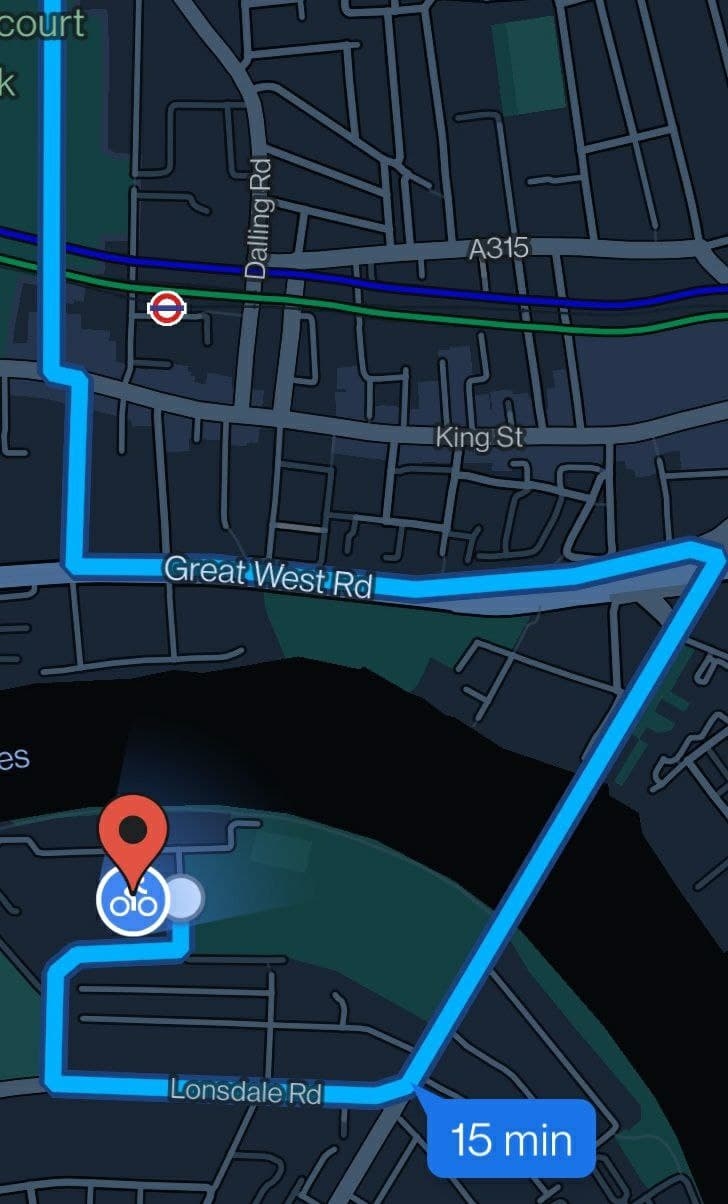
\includegraphics[height=5cm]{route.jpg}
    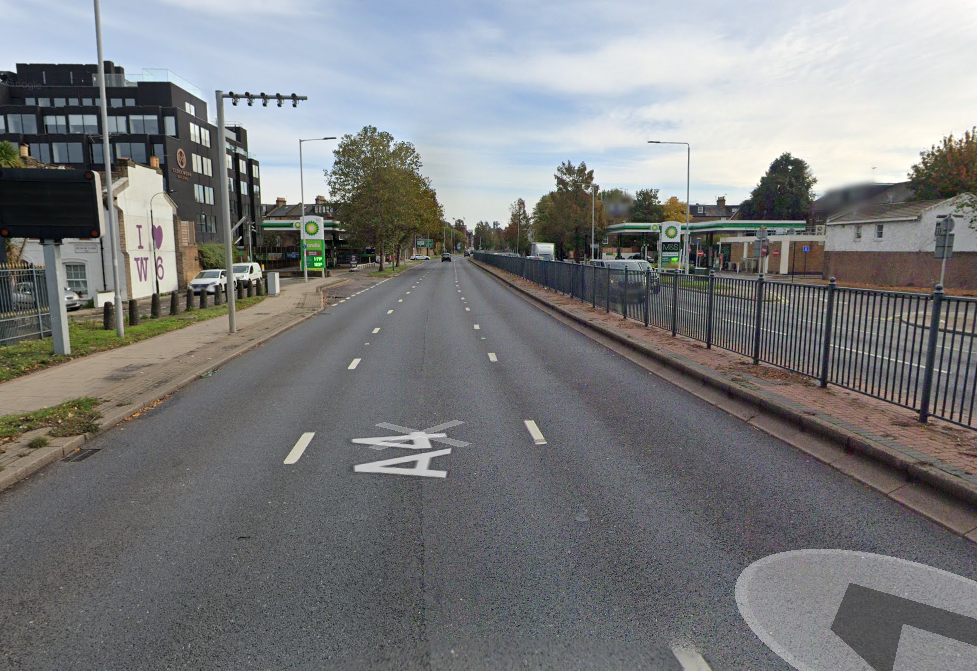
\includegraphics[height=5cm]{dangerous.png}
\end{center}
    \caption{Route suggested by google maps}
    \label{route}
\end{figure}
However many of these route finding applications don't take into account safety. This is shown in Figure \ref{route} which shows the route Google Maps suggests that I cycle to school by. The route includes the A4, which is a very dangerous stretch of road for cyclists as it is a 3 lane road. 
My plan is to combine accident statistics with traffic data to work out which roads are dangerous and then avoid them (finding the least dangerous instead of the shortest route).
\subsection{Client}
The client is me because I am personally not a fan of being involved in cycling accidents
\subsection{Similar Systems}
There exist similar systems such as google maps and Citymapper. These have advantage's over me such as being able to use live traffic data and other such things. Citymapper has a option to choose between "Quiet", "Regular", and "Fast" routes, which seems to be based on the type of road you are taken down.
However they don't really take accident density into account which will be my aims.
\subsection{Features}
\subsection{Map data}
I need a data source which can provide data on roads that are legal to cycle on as well as being freely available for me to use. I settled on Open Street Map, a project which combines data gathered by volunteers into one massive freely available map. The map is downloadable in the form of a large XML file or PBF file. A PBF file is just a binary version of the same thing. I could write code to parse this myself, but instead I think that I am going to use the library libosmium
which works in C++.
\subsection{Accident Data}
\begin{figure}
    \begin{center}
        \begin{tikzpicture}[scale=1]
        \draw[gray, thick] (-4,0) -- (4,0);
        \draw[gray, thick] (0,-4) -- (0,4);
        \filldraw[black] (0,0) circle (2pt) node[anchor=west]{};
        \filldraw[black] (0,2) circle (2pt) node[anchor=west]{};
        \filldraw[black] (2,0) circle (2pt) node[anchor=west]{};
        \filldraw[black] (-2,0) circle (2pt) node[anchor=west]{};
        \filldraw[black] (0,-2) circle (2pt) node[anchor=west]{};
\filldraw[black] (0,-4) circle (2pt) node[anchor=west]{};
\filldraw[black] (0,4) circle (2pt) node[anchor=west]{};
\filldraw[black] (4,0) circle (2pt) node[anchor=west]{};
\filldraw[black] (-4,0) circle (2pt) node[anchor=west]{};
    \end{tikzpicture}
\end{center}
    \caption{Typical OSM representation of an intersection}
    \label{intersection}
\end{figure}
Transport for London has an excellent API which you can download accident data from. The data comes in JSON files and contains information about what type of vehicle was involved in each accident, the severity, and the coordinates of the accident. 
I need to find a way of mapping the coordinates onto the road network so that the danger of roads can be calculated as accurately as possible. Originally I was looking at adding the accident to the nearest edge in the graph but I decided against this after considering how intersections 
are typically represented in OSM. Road intersections typically look something like what is represented in Figure \ref{intersection}. If an accident were to occur at the intersection it would end up being added to one of the segments leading into the intersection, so the danger would not be properly calculated if not passing through that segment. Instead I thought about adding the danger to the nearest node, so that the accident would always be counted when a route passes through that intersection.
The other problem that I have to deal with, if adding data to the nearest node is that the density of nodes is not constant. Straighter roads will not need to use as many OSM nodes as curved roads, so i might incorrectly add cost to the wrong node. My proposed solution to this is to interpolate in nodes to a very high density to deal with this problem.
\subsection{Traffic Data}
The main problem with this is that the accident data is absolute and can thus not be used to calculate probabilities. For example, more accidents happen on King's Street than the dangerous road I showed earlier, but this doesn't mean that King's Street is more dangerous merely that more cyclists travel on it. This means that I need to get accurate cyclist traffic data for the whole of London in order to turn my accident statistics into accident probabilities.
The Department for Transport and the Office for National Statistics both keep data on traffic, but it isn't applicable because cycle data is only given as a total \footnote{0.6 billion miles per year in London} and at specific count points.
This means that I will either need to work out traffic data or get it from some dataset, such as Strava's Global Heatmap. \\
Luckily the rest of the application can work without including traffic data so my plan is to deal with this problem at a later time.  \label{end}
\subsection{Finding the shortest route}
Dijkstra's algorithm and A* are both very slow. I will use preprocessing based algorithms such as ALT* to make my program run a lot faster.
\subsection{Critical Path}
\begin{itemize}
    \item Import accidents
    \item Match accidents to nodes
    \item Build Graph
    \item Write pathfinder algorithms
\end{itemize}
\end{document}
